\documentclass[12pt, oneside]{amsart}
\usepackage{geometry}                % See geometry.pdf to learn the layout options. There are lots.
\geometry{letterpaper}                   % ... or a4paper or a5paper or ... 
\usepackage[superscript]{cite}
%\geometry{landscape}                % Activate for for rotated page geometry
%\usepackage[parfill]{parskip}    % Activate to begin paragraphs with an empty line rather than an indent
\usepackage{graphicx}
\usepackage{amssymb}
\usepackage{epstopdf}
\usepackage{setspace}
\usepackage{float}
\usepackage{caption}
\usepackage{subcaption}

\usepackage{algpseudocode}

%Code Highlighting
\usepackage{listings}
\usepackage{color}
\definecolor{dkgreen}{rgb}{0,0.6,0}
\definecolor{gray}{rgb}{0.5,0.5,0.5}
\definecolor{mauve}{rgb}{0.58,0,0.82}

\lstset{ %
  backgroundcolor=\color{white},  % choose the background color; you must add \usepackage{color} or \usepackage{xcolor}
  basicstyle=\footnotesize,       % the size of the fonts that are used for the code
  breakatwhitespace=false,        % sets if automatic breaks should only happen at whitespace
  breaklines=true,                % sets automatic line breaking
  captionpos=b,                   % sets the caption-position to bottom
  commentstyle=\color{dkgreen},   % comment style
 % frame=single,                   % adds a frame around the code
  keywordstyle=\color{blue},      % keyword style
  language=Python,                % the language of the code
  morekeywords={*,...},           % if you want to add more keywords to the set
  numbers=left,                   % where to put the line-numbers; possible values are (none, left, right)
  numbersep=5pt,                  % how far the line-numbers are from the code
  numberstyle=\tiny\color{gray},  % the style that is used for the line-numbers
  rulecolor=\color{black},        % if not set, the frame-color may be changed on line-breaks within not-black text (e.g. comments (green here))
  showspaces=false,               % show spaces everywhere adding particular underscores; it overrides 'showstringspaces'
  showstringspaces=false,         % underline spaces within strings only
  showtabs=false,                 % show tabs within strings adding particular underscores
  stepnumber=1,                   % the step between two line-numbers. If it's 1, each line will be numbered
  stringstyle=\color{mauve},      % string literal style
  tabsize=2,                      % sets default tabsize to 2 spaces
}


\usepackage{url}
%\onehalfspacing
\DeclareGraphicsRule{.tif}{png}{.png}{`convert #1 `dirname #1`/`basename #1 .tif`.png}

\title{Reducing The Impact of Cliques in Social News Sites}
\author{Ed Kelley, DJ Shuster, Brian Matejek}
\date{15 January 2013}         % Activate to display a given date or no date

\begin{document}
\begin{center}
% \includegraphics[scale=.075]{branch-logo.jpg}
\end{center}
\maketitle

% Background and Motivation
\section{Motivation}
In 2004, Digg launched as one of the first  popularity-based news sites on the Web. Instead of just a content delivery site, Digg was a platform where any user could submit a story and users voted to determine the order of the displayed stories. In the following years, similar sites, such as Reddit, StumbleUpon, and Hacker News, have seen a huge rise in popularity.

However, due to the nature of their voting systems, these sites are highly susceptible to collusion. There have been several instances of small groups of users, typically with strong political affiliations, colluding to ``bury" or ``downvote" content they disagree with and ``digg" or ``upvote" content that aligns with their politcal views. In 2007, Muhammad Saleem, a researcher for the Search Engine Journal, published an article titled  ``The Bury Brigade Exists, and Here's My Proof," showing that there were groups of users on Digg which were ``hard at work burying any content that doesn't suit [their] ideology."\cite{wired, sej}

Later, in 2010, AltNet published a story about the ``Digg Patriots," a small group of conservative users that were ``able to bury over 90\% of the articles by certain users and websites submitted within 1-3 hours" and promote their own stories to the front page.\cite{alter net} These users would gather on Yahoo Groups in order to collude on their voting.

This behavior was not limited to Digg. In 2012, The Daily Dot published a story about ``LibertyBot," a bot that would use many accounts to downvote any posts seen as anti-libertarian or, more specifically, anti-Ron Paul.\cite{dailydot} These small groups of users are having a disproportionate impact on the content displayed on the front page of these social news sites.

\section{Goal}

Our goal is to find an algorithm that will reduce the impact of these cliques on the ranking of stories. This algorithm must be able to perform online with a large number of users and posts. Additionally, this algorithm should produce a ranking that places the most highly voted stories to the top, while diminishing the influence of biased cliques.

\section{Reddit Ranking Algorithm}

For comparison, we will be using the Reddit ``Hot" Ranking algorithm. This algorithm assigns a a rating for each post which takes into account the difference between upvotes and down votes as well as the age of the post.

\begin{figure}[h]
	\centering
	\begin{algorithmic}[1]
	\State $s \gets (ups-down)$
	\State $order \gets \log_{10}{\lvert s \rvert}$ \Comment{By taking log, increase impact of early votes}
	\If {$order < 1$}
		\State $order \gets 1$
	\EndIf
	\If {$s > 0$}
		\State $sign \gets 1$
	\ElsIf{$s < 0$}
		\State $sign \gets -1$
	\Else
		\State $sign \gets 0$
	\EndIf
	\State $seconds \gets (now - 1134028003)$ \Comment{Time since an arbitrary date in 2005}
	\State \Return $order + \frac{sign * seconds}{45000}$  \Comment{45000 seconds = 12.5 hours}
	\end{algorithmic}
	\caption{Pseudocode of Reddit's ``Hot" Ranking Algorithm}

\end{figure}

\section{Strategies}

\subsection{Noisy Ranking}
The Gibbard-Satterthwaite Theorem expresses the idea that all deterministic voting rules are either dictatorial or non-strategy-proof. This means that either a single individual has the power to decide the entire election, or all agents have the incentive to lie about their true preferences. Neither of these scenarios is particularly attractive in a democratic selection process, a fact that has driven discussion toward the design of more favorable voting mechanisms.


One particular strategy, set forth originally by Gibbard and extended more recently by Conitzer and Sandholm, is the use of mechanisms that use randomized approximations\cite{birrell}. These mechanisms are meant to mimic deterministic voting rules while adding a certain component of randomness. However, Gibbard also showed that these rules may only become strategy-proof in trivial scenarios. Nevertheless, the true advantage of this line of thinking is that it allows for the potential to develop voting mechanisms that may be considered �approximately strategy-proof�. Birrell and Pass first developed this term to accomodate the phenomenon that individuals tend to report their preferences honestly when tactical voting provides only a small benefit. Birrell and Pass explain this phenomenon by postulating that there exists a psychological cost to lying. For this discussion, allow this value to be defined as epsilon. For a given value of epsilon, a voting rule is defined as being �approximately strategy-proof� if the benefit of misrepresentation is less than epsilon.\cite{birrell}


Using these definitions as a framework, we sought to develop suitable randomized approximations of existing content-ranking algorithms. The first, and most simple, and of these voting rules involves adding noise to the voting process. Essentially, the algorithm introduces a certain probability of reversing each vote every time the post�s score is reported. While this strategy may seem very simple, it provides an effective measure for combatting collusion. To begin, consider 3 types of users and posts (unbiased, bias1, bias2). Unbiased users upvote or downvote all posts using the same probability distributions, regardless of the posts� biases. On the other hand, biased users will favor posts of their own bias, upvoting them with much higher probability than other posts. They are also much more likely to downvote posts that do not share their bias. Once noise is introduced, there is a certain probability that the user�s vote will counted in the opposite direction. Effectively, this reduces the overall benefit the user receives from casting his or her vote, as it is uncertain whether or not it will be cast favorably.


By following this line of thinking, noisy voting may also be a way to reduce the benefit received by mischaracterizing the user�s preferences. In our model, this reflects the undesirable effect of collusion. By adding noise, it is possible that the benefit of collusion may be brought below the epsilon value required for a voting rule to become �approximately strategy proof �. Another way to think of this effect is to see that the noise is effectively altering the user�s voting probability functions. In the simulations that we have run, unbiased users ignore a post with 60\% probability, upvote it with 25\% probability and downvote with 15\% probability. Essentially, the expected score for any post is $.1 * n_{unbiased}$. Biased users, however, have only a 2\% probability of ignoring a post with the same bias and a 2\% probability of downvoting it, but a 96\% probability of upvoting it. So, a biased post has an expected score of $.94 * n_{same bias}$. When viewing any other post, the biased users have a 40\% probability of ignoring it, a 40\% probability of downvoting it, and a 20\% probability of upvoting it. This means that any post has an expected score of $-.2 * n_{different bias}$. If there are two groups of biased individuals, each post will have the following expected scores:




\begin{align}
E(unbiased post) &= .1 * n_{unbiased} - .2 * n_{bias 1} - .2 * n_{bias 2}\\
E(bias 1 post) &= .1 * n_{unbiased} + .94 * n_{bias 1} - .2 * n_{bias 2}\\
E(bias 2 post) &= .1 * n_{unbiased} - .2 * n_{bias 1} + .94 * n_{bias 2}\\
Var(unbiased post) &= .384 * n_{unbiased}^{2} + .544 * n_{bias 1}^{2} + .544 * n_{bias 2}^{2}\\
Var(bias 1 post) &= .384 * n_{unbiased}^{2} + .079 * n_{bias 1}^{2} + .544 * n_{bias 2}^{2}\\
Var(bias 2 post) &= .384 * n_{unbiased}^{2} + .544 * n_{bias 1}^{2} + .079* n_{bias 2}^{2}
\end{align}




Clearly, biased posts will always have the upper hand in this scenario. However, noisy voting helps to combat this effect. Once noise is introduced, and there is a 20\% probability for votes to be altered, unbiased users will still have a 60\% probability of ignoring a post, but will instead have a 23\% probability of having their vote recorded as an upvote and a 17\% probability of having their vote recorded as a downvote. This makes each post�s expected score equal to $.06 * n_{unbiased}$. Biased users will still have a 2\% probability of ignoring a post of their own bias, but will instead have a 77.2\% probability of having their vote recorded as an upvote and 20.8\% chance of having it be recorded as a downvote. Now, a biased post will have an expected score of $.564 * n_{same bias}$. In addition, biased users will still have a 40\% probability of ignoring a post with a different bias, but only a 36\% probability of having their vote be recorded as a downvote and a 24\% chance of having it recorded as an upvote. Now, any post will have an expected score of $-.12 * n_{different bias}$. If there are two groups of biased individuals, each post will have the following expected scores:


\begin{align}
E(unbiased post) &= .06 * n_{unbiased} - .12 * n_{bias 1} - .12 * n_{bias 2}\\
E(bias 1 post) &= .06 * n_{unbiased} + .564 * n_{bias 1} - .12 * n_{bias 2}\\
E(bias 2 post) &= .06 * n_{unbiased} - .12 * n_{bias 1} + .564 * n_{bias 2}\\
Var(unbiased post) &= .394 * n_{unbiased}^{2} + .580 * n_{bias 1}^{2} + .580 * n_{bias 2}^{2}\\
Var(bias 1 post) &= .394 * n_{unbiased}^{2} + .645 * n_{bias 1}^{2} + .580 * n_{bias 2}^{2}\\
Var(bias 2 post) &= .394 * n_{unbiased}^{2} + .580 * n_{bias 1}^{2} + .645* n_{bias 2}^{2}
\end{align}


Once noise is introduced, all expected scores decrease, while variances of expected scores increase. While the expected scores decrease in equal proportions for both biased and unbiased posts, the variance of biased posts increases relatively greater than that of unbiased posts. However, since these probability distribution functions are not normal, we must plot them in order to achieve a full understanding of the results.

\begin{figure}
	\centering
	\begin{subfigure}[b]{0.5\textwidth}
		\centering
		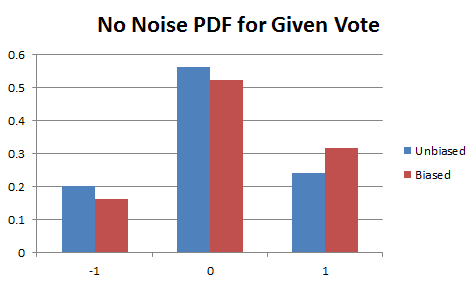
\includegraphics[width=\textwidth]{images/no_noise_graphic.png}
		\caption{No Noise}
	\end{subfigure}%
	\begin{subfigure}[b]{0.5\textwidth}
		\centering
		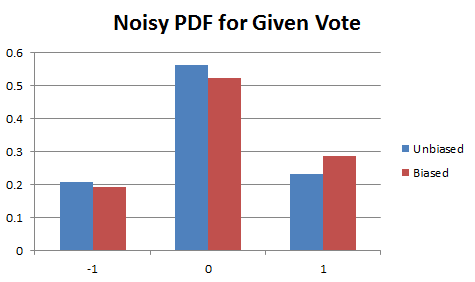
\includegraphics[width=\textwidth]{images/noisygraphic.png}
		\caption{With Noise}
	\end{subfigure}
\end{figure}

Once the results are plotted, it appears that the added noise causes the biased and unbiased distributions to converge. Ultimately, this leads to a lesser likelihood for biased posts to appear on the front page than in the noseless case.

\subsection{Sampling}
Another method for collusion resistance is inspired by 'lottery voting'.\cite{amar} This voting mechanism works by choosing voters at random amongst a given population. These chosen few then cast ballots and determine the result of the election. While this sounds like a fairly radical idea, it is quite similar to the American jury system used to determine the guilt of an accused criminal on behalf of the people. In practice, lottery voting is believed to have several significant impacts on elections dynamics.\cite{amar} Since each individual vote has the potential to count for for a far greater share of the decision than in a traditional election, voters have the incentive to make more carefully reasoned decisions. In addition, lottery voting has a much more positive effect on maintaining proportional representation and cross-sectionalism in the voting group.\cite{amar} With this voting system, the choices of the minority actually matter and aren't simply dismissed by the majority as they are in our current "first past the pole" voting system. This also has the effect of increasing the viability of third party candidates that more accurately reflect a voter's preferences. In essence, lottery voting has the potential to be more truthful than traditional voting mechanisms.


As with the noisy case above, lottery voting is also a randomized approximation of a deterministic voting rule. Again, this allows us to explore the possibility for "approximate strategy-proofness". In our case, the algorithm works by first recording all upvotes and downvotes as normal. Then, each time the post's score is reported, the algorithm will randomly sample a portion of the post's votes. Then, this sample is extrapolated to represent the full volume of the post's votes. As with the lottery voting system, this sampling method allows for more accurate representation on the front page. Now, the percentage of unbiased posts on the front page should be more indicative of the total percentage of votes cast for unbiased posts. This should reduce the positive benefit brought on by the collusive groups' tendency to cause biased posts to have slightly higher expected scores.

\section{Simulations}

We simulated the data over what would be an equivalent of 1 day, with 100, 300, and 1000 users.  The simulations creates posts every minute and go throughs all of the users.  The users can look at the last 3 hours worth of posts on the website (since users would rarely in real life go through many more posts than this).  Users can either consciously not vote, up vote, or down vote a post.  Once the user does this, the user will never vote again on the same post.  Every thirty minutes the page rank algorithms of Reddit, Noisy, and Sampling are called which determine which pages make the front page.  Front page is formally defined as the top 30 posts at any given time on our simulated social content website.  The number of biased posts that make the front page is calculated for each of the simulations, and the following section describes proofs from this data.

We also ran simulations where there was only one collusive group.  In 2010, the website Digg discovered a group of users called the Digg Patriots who gained a disproportionate amount of influence over the content of the website.  We also looked at how our modified page rank algorithms handled this situation.

\section{Analysis}

We can form a binomial distribution of posts on the front page. The front page is calculated 47 times during the course of the simulation, and 30 posts are on each front page. If a post in a given slot on the front page is not biased, a random variable receives the value 1, otherwise it gets the value 0. Our null hypothesis ($H_0$) is that collusive groups or cliques do not have excessive influence on getting posts to the front page. Our alternative hypothesis ($H_A$) is that collusive groups do have excessive influence in getting posts to the front page. We will start by looking at the case where there are 100 users, 5 belong to one clique, 5 to another, and 85\% of posts are not biased one way or the other. For $H_0$:
\begin{center}
$H_0: \mu \geq 1198.5$\quad$H_A: \mu < 1198.5$ \\
n = 1410 \quad p = .85 \\
$\mu = np = 1410 (.85) = 1198.5$ \quad $\sigma^2 = np(1 - p) = 1410 (.85)(.15) = 179.8$ \\
\end{center}
After 50 trials with 100 users:
\begin{center}
$\mu_{reddit} = 766$ \quad $\mu_{sampling} = 1004$ \quad $\mu_{noisy} = 947$
\end{center}
$$SE = \sqrt{\frac{\sigma^2}{n}} = \sqrt{\frac{179.8}{50}} = 1.896$$
\begin{center}
$Z_{reddit} = \frac{1198.5 - 766}{1.896} = 228.4$ \quad $Z_{sampling} = \frac{1198.5 - 1004}{1.896} = 102.6$ \quad $Z_{noisy} = \frac{1198.5 - 947}{1.896} = 132.7$
\end{center}
All three of these Z-indexes confirm that with 100 users, and 10 belonging to cliques, we can confidently replace the null hypothesis with the alternative hypothesis. Even with our algorithms, the probability of belonging to a clique is too great that the front page is still overly populated with their posts. However, noisy and sampling still do better than Reddit in terms of preventing posts from cliques from filling up the front page. For the following proofs, the null hypothesis ($H_0$) is that there is no difference in preventing cliques posts between the Reddit and sampling/noisy algorithms. The alternative hypothesis ($H_A$) is that sampling/noisy does better than Reddit. The means were determined for each of the 50 runs. We can create a $\mu_{diff}$ by subtracting means from the same run. First we will compare the Reddit and sampling algorithms.
\begin{center}
$H_0: \mu_{reddit} = \mu_{sampling}$ \quad $H_A: \mu_{reddit} < \mu_{sampling}$ \\
$\mu_{diff} = 19.8$ \quad $\sigma_{diff} = 73.24$ \quad $SE_{diff} = 10.36$ \\
$Z_{diff} = \frac{19.8 - 0}{10.36} = 1.91$ \\
\end{center}
We can say with over 97\% confidence that the null hypothesis is wrong and that sampling works better than the reddit algorithm.
\vspace{.2cm}
Next, we will compare the reddit and noisy algorithms.
\begin{center}
$H_0: \mu_{reddit} = \mu_{noisy}$ \quad $H_A: \mu_{reddit} < \mu_{noisy}$ \\
$\mu_{diff} = 15.05$ \quad $\sigma_{diff} = 55.81$ \quad $SE_{diff} = 7.89$ \\
$Z_{diff} = \frac{15.05 - 0}{7.89} = 1.91$ \\
\end{center}
We can say with over 97\% confidence that the null hypothesis is wrong and that sampling works better than the reddit algorithm.
\vspace{.2cm}
Lastly, we will compare the sampling and noisy algorithms, with the alternative hypothesis that the sampling algorithm is better than the noisy algorithm.
\begin{center}
$H_0: \mu_{noisy} = \mu_{sampling}$ \quad $H_A: \mu_{noisy} < \mu_{sampling}$ \\
$\mu_{diff} = 4.75$ \quad $\sigma_{diff} = 18.37$ \quad $SE_{diff} = 2.60$ \\
$Z_{diff} = \frac{4.75 - 0}{2.60} = 1.83$ \\
\end{center}
The p-value for this test is .0336, so we can say with over 96\% confidence that sampling is better than the reddit algorithm.
\vspace{.4cm}
We also did two other tests (with 300 and 1000 users), and varied the number of users belonging to cliques. For the test with 300 users, we had 5\% of users belonging to two different cliques (2.5\% in each) and 4\% of posts belonging to cliques. First, to see if colluding groups have disproportionate amount of influence (the alternative and null hypotheses are the same). The expected number of posts on the front page belonging to cliques is:
\begin{center}
n = 1410 \quad p = .96 \\
$\mu = np = 1410 (.96) = 1353.6$ \quad $\sigma^2 = np(1 - p) = 1410 (.96)(.04) = 54.14$ \\
$H_0: \mu \geq 1353.6$ \quad $H_A: \mu < 1353.6$ \\
\end{center}
\begin{center}
$\mu_{reddit} = 1236$ \quad $\mu_{sampling} = 1301$ \quad $\mu_{noisy} = 1286$ \\
$SE = \sqrt{\frac{\sigma^2}{n}} = \sqrt{\frac{54.14}{50}} = 1.041$ \\
$Z_{reddit} = \frac{1353.6 - 1236}{1.041} = 112.97$ \quad $Z_{sampling} = \frac{1353.6 - 1301}{1.041} = 50.53$ \quad $Z_{noisy} = \frac{1353.6 - 1286}{1.041} = 64.94$ \\
\end{center}
These z-indexes are large enough that we can conclude that colluding groups still have a disproportionate amount of influence. However, again we want to see which (if any) of these algorithms is the best. We will start by comparing the sampling and Reddit algorithms. Our null hypothesis is that Reddit and sampling are comparable, and our alternative hypothesis is that sampling is better.
\begin{center}
$H_0: \mu_{reddit} = \mu_{sampling}$ \quad $H_A: \mu_{reddit} < \mu_{sampling}$ \\
$\mu_{diff} = 5.39$ \quad $\sigma_{diff} = 20.1$ \quad $SE_{diff} = 2.84$ \\
$Z_{diff} = \frac{5.39 - 0}{2.84} = 1.90$ \\
\end{center}
We can assert with over 97\% confidence that our null hypothesis is wrong and the alternative, that sampling is better than Reddit's algorithm.
\vspace{.2cm}
Next, we will compare the Reddit and noisy ranking algorithms, with our null and alternative hypotheses the same as above.
\begin{center}
$H_0: \mu_{reddit} = \mu_{noisy}$ \quad $H_A: \mu_{reddit} < \mu_{noisy}$ \\
$\mu_{diff} = 4.15$ \quad $\sigma_{diff} = 15.81$ \quad $SE_{diff} = 2.24$ \\
$Z_{diff} = \frac{4.15 - 0}{2.24}= 1.85$ \\
\end{center}
This gives a p-value of .0322, so we can say with over 96\% confidence that the noisy algorithm is better than the reddit algorithm with 300 users.
\vspace{.2cm}
Lastly, we will compare the sampling and noisy algorithms, with our null and alternative hypotheses the same as above.
\begin{center}
$H_0: \mu_{noisy} = \mu_{sampling}$ \quad $H_A: \mu_{noisy} < \mu_{sampling}$ \\
$\mu_{diff} = 1.24$ \quad $\sigma_{diff} = 5.58$ \quad $SE_{diff} = .79$ \\
$Z_{diff} = \frac{1.24 - 0}{.79} = 1.57$ \\
\end{center}
This gives a p-value of over .05. We cannot therefore conclude that the sampling algorithm is better than the noisy algorithm with 95\% confidence. For 300 users, we do not have conclusive evidence if sampling or noisy is a better algorithm.
\vspace{.4cm}
We did an additional test with 1000 users, where the probability of any given post being biased is 96\%. Again, we start by determining if collusive groups have a disproportionate amount of influence over the content that reaches the front page. First, to see if colluding groups have disproportionate amount of influence (the alternative and null hypotheses are the same):
\begin{center}
n = 1410 \quad p = .96 \\
$\mu = np = 1410 (.96) = 1353.6$ \quad $\sigma^2 = np(1 - p) = 1410 (.96)(.04) = 54.14$ \\
$H_0: \mu \geq 1353.6$ \quad $H_A: \mu < 1353.6$ \\
$\mu_{reddit} = 1140$ \quad $\mu_{sampling} = 1253$ \quad $\mu_{noisy} = 1228$ \\
$SE = \sqrt{\frac{\sigma^2}{n}} = \sqrt{\frac{54.14}{50}} = 1.041$ \\
$Z_{reddit} = \frac{1353.6 - 1140}{1.041} = 205.2$ \quad $Z_{sampling} = \frac{1353.6 - 1253}{1.041} = 96.64$ \quad $Z_{noisy} = \frac{1353.6 - 1228}{1.041} = 120.65$ \\
\end{center}
These z-indexes also show that collusive groups still have a considerable influence on what content makes the front page. Next, as above, we will determine if either of these two new algorithms is more successful in keeping the front page free of biased content. We will start by comparing the sampling and Reddit algorithms. Our null hypothesis is that Reddit and sampling are comparable, and our alternative hypothesis is that sampling is better:
\begin{center}
$H_0: \mu_{reddit} = \mu_{sampling}$ \quad $H_A: \mu_{reddit} < \mu_{sampling}$ \\
$\mu_{diff} = 9.39$ \quad $\sigma_{diff} = 33.25$ \quad $SE_{diff} = 4.70$ \\
$Z_{diff} = \frac{9.39 - 0}{4.70} = 2.00$ \\
\end{center}
We can assert with over 97\% confidence that our null hypothesis is wrong and the alternative, that sampling is better than Reddit's algorithm.
\vspace{.2cm}
Next, we will compare the Reddit and noisy ranking algorithms, with our null and alternative hypotheses the same as above.
\begin{center}
$H_0: \mu_{reddit} = \mu_{noisy}$ \quad $H_A: \mu_{reddit} < \mu_{noisy}$ \\
$\mu_{diff} = 7.36$ \quad $\sigma_{diff} = 26.25$ \quad $SE_{diff} = 3.71$ \\
$Z_{diff} = \frac{7.36 - 0}{3.71} = 1.98$ \\
\end{center}
We can say with over 97\% confidence that the noisy algorithm is better than the reddit algorithm with 300 users.
\vspace{.2cm}
Lastly, we will compare the sampling and noisy algorithms, with our null and alternative hypotheses the same as above.
\begin{center}
$H_0: \mu_{noisy} = \mu_{sampling}$ \quad $H_A: \mu_{noisy} < \mu_{sampling}$ \\
$\mu_{diff} = 2.02$ \quad $\sigma_{diff} = 7.99$ \quad $SE_{diff} = 1.13$ \\
$Z_{diff} = \frac{2.02 - 0}{1.13} = 1.79$ \\
\end{center}
This gives a p-value just under .04. We can therefore justify saying that the sampling algorithm better eliminates the influence of cliques then the noisy algorithm.

\section{Discussion and Conclusion}

Social content sites are susceptible to collusive groups that try to manipulate which posts reach the front page.  Even with the two methods that are collusion resistant, groups can still gain a disproportionate number of front page posts.  The trouble arises from the fact the algorithms are run online - the interactions between users and how they will vote in the future are unknown.  In our voting schemes, all the votes are tallied at once, but on a social content website, votes come in at different intervals.  A page might make the front page shortly after being posted, with less than 10\% of the total websites users seeing the content.  Another issue with collusive groups is that their members tend to vote in force - on both posts that favor and oppose their opinions.  Casual users of a social content website vote on fewer articles, which gives the collusive group even more power over the content of the front page.  Our simulation takes this into consideration when determining how user's voted on content.  In conclusion, Reddit's algorithm does not sufficiently offer protection against colluding groups or cliques of people.  Users can gain a disproportionate amount of influence over the content of the front page, particularly the front pages of smaller subreddits. Both of the techniques we implemented were able to partially mitigate the influence of these groups.

\section{Suggestions for Future Work}

One of the aspects that we did not fully study was the \emph{quality} of posts that reach the front page. That is, we carefully studied the distribution of biased vs. unbiased posts which reached the front page, but did not keep track of any ``total front page score" based on the truthful views of unbiased users. By the criteria of biased vs. unbiased posts, an effective algorithm would be to just randomly chose the stories on the front page. However, this algorithm would not result in a high quality front page. Essentially, there is a tradeoff that should be studied between the attempts to reduce collusion and the desire to have a high quality front page.

\newpage

\section{Appendix}

\subsection{main.py}
Creates users and posts, runs simulation, and prints results.
 
\lstinputlisting{../main.py}


\newpage

\subsection{user.py}
User class. Contains voting logic.

\lstinputlisting{../user.py}

\newpage

\subsection{post.py}
Post class. 

\lstinputlisting{../post.py}

\newpage

\subsection{reddit.py}
Actual Reddit ranking algorithm.

\lstinputlisting{../reddit.py}

\newpage

\subsection{noisy.py}
Noisy algorithm.

\lstinputlisting{../noisy.py}

\newpage

\subsection{sampling.py}
Sampling algorithm.

\lstinputlisting{../sampling.py}


\newpage
\nocite{*}
\bibliography{bib}{}
\bibliographystyle{plain}

\vfill
This paper represents our own work in accordance with university regulations.


\end{document}  